
O \textit{standard} ISO/IEC (\textit{International Organization for Standardization} / \textit{International Electrotechnical Commission}) 18013 é caracterizado pelo título geral \texttt{Personal Identification} -- \texttt{ISO
Compliant Driving Licence} e é constituído pelas seguintes partes:

\begin{itemize}
	\item \textbf{Parte 1} -- \texttt{Physical Characteristics and Basic Data Set} \cite{iso_1}: descreve as características físicas, o conjunto básico de elementos de dados, o \textit{layout} visual e as capacidades de segurança física (recursos legíveis pelo ser humano) de uma \textit{ISO-compliant driving licence} (IDL);
	\item \textbf{Parte 2} -- \texttt{Machine-Readable Technologies} \cite{iso_2}: descreve as tecnologias, legíveis por máquina, que podem ser utilizadas por este \textit{standard}, incluindo a estrutura de dados lógica e o mapeamento de dados por cada tecnologia;
	\item \textbf{Parte 3} -- \texttt{Access Control, Authentication and Integrity Validation} \cite{iso_3}: descreve as capacidades de segurança eletrónica que podem incorporar este \textit{standard}, incluindo mecanismos para controlo de acesso aos dados, verificação da origem de uma IDL e confirmação da integridade dos dados;
	\item \textbf{Parte 4} -- \texttt{Test Methods}: descreve métodos de teste que podem ser utilizados para determinar se uma IDL está de acordo com os requisitos das tecnologias legíveis por máquinas especificadas na parte 2 e com as capacidades de segurança eletrónica especificadas na parte 3.
\end{itemize}

Este \textit{standard} cria uma base comum para a utilização internacional e reconhecimento mútuo da IDL, sem impedir que países ou estados apliquem as suas regras de privacidade e que autoridades nacionais/comunitárias/regionais de trânsito tratem das suas necessidades específicas.

A \textbf{Parte 5} do ISO/IEC 18013 -- \texttt{Mobile Driving Licence} \cite{iso_5} -- pretende estabelecer um \textit{standard} de especificações de interface para a implementação de cartas de condução associadas a dispositivos móveis (\textit{Mobile Driving License} - mDL). Assim, esta parte descreve a interface e requisitos físicos e funcionais associados, que possibilitam a utilização de dispositivos móveis pelo titular da carta de condução, para a fornecer a um verificador, facilitando o acesso do mesmo a informação da carta de condução.

Neste contexto, considera-se que dispositivos móveis são os dispositivos eletrónicos com interface de utilizador e a capacidade de armazenar informação da mDL e de a partilhar com um leitor, após instrução do titular -- \textit{smartphones}, \textit{wearables}, entre outros. Um leitor mDL é um dispositivo portátil ou computador, que pode trocar dados com uma mDL, enquanto que o titular da mDL é o indivíduo para quem a mDL é emitida, isto é, o titular legítimo dos privilégios de condução refletidos na mDL.

O objetivo do ISO/IEC 18013-5 é permitir que verificadores não associados à autoridade de emissão da mDL, como outras autoridades de emissão ou entidades verificadoras de outros países, ganhem acesso à informação para a qual o titular da mDL providenciar consentimento, conseguindo autenticá-la. Para o conjunto de informações disponibilizado pelo titular da mDL, estas entidades deverão poder:

\begin{enumerate}
	\item Utilizar uma máquina para obter a informação da mDL;
	\item Estabelecer a conexão entre a mDL e o seu titular, com um grau aceitável de confiança;
	\item Autenticar a origem da informação da mDL;
	\item Verificar a integridade da informação da mDL.
\end{enumerate}

Salienta-se a utilidade do titular poder aceder e facultar dados da sua carta de condução através de um dispositivo móvel, sendo este tipo de dispositivos muito utilizado atualmente. Outra vantagem das mDL em relação às cartas de condução físicas é a capacidade de atualizar informação com mais frequência e autenticá-la com um nível de confiança superior.

Existem três interfaces fulcrais para esta parte do \textit{standard}, que são explicadas de seguida:

\begin{enumerate}
	\item Interface entre a mDL e a autoridade emissora, que permite controlar, entre outros, como a mDL é fornecida e como são efetuadas atualizações. Esta interface não é o foco desta parte do ISO/IEC 18013, uma vez que a interoperabilidade entre autoridades emissoras não é requerida para as funcionalidades pretendidas.
	\item Interface entre a mDL e o leitor, que tem de funcionar em tempo real e é descrita na parte 5 do ISO/IEC 18013.
	\item Interface entre a autoridade emissora e a entidade de verificação, que facilita a troca de informação requerida para permitir a um leitor confirmar a autenticidade da informação da mDL e, em alguns casos, ler alguma informação da mesma. Esta interface é estabelecida preferencialmente entre a entidade verificadora e a autoridade emissora (diretamente ou através de intermediários), em vez de diretamente entre o leitor e a autoridade de emissão. Para além disso, não precisa de funcionar em tempo real e pode ser usada pela própria autoridade emissora, em leitores sob o seu controlo. Esta interface é descrita nesta parte do ISO/IEC 18013.
\end{enumerate}

\begin{figure}[H]
	\centering
	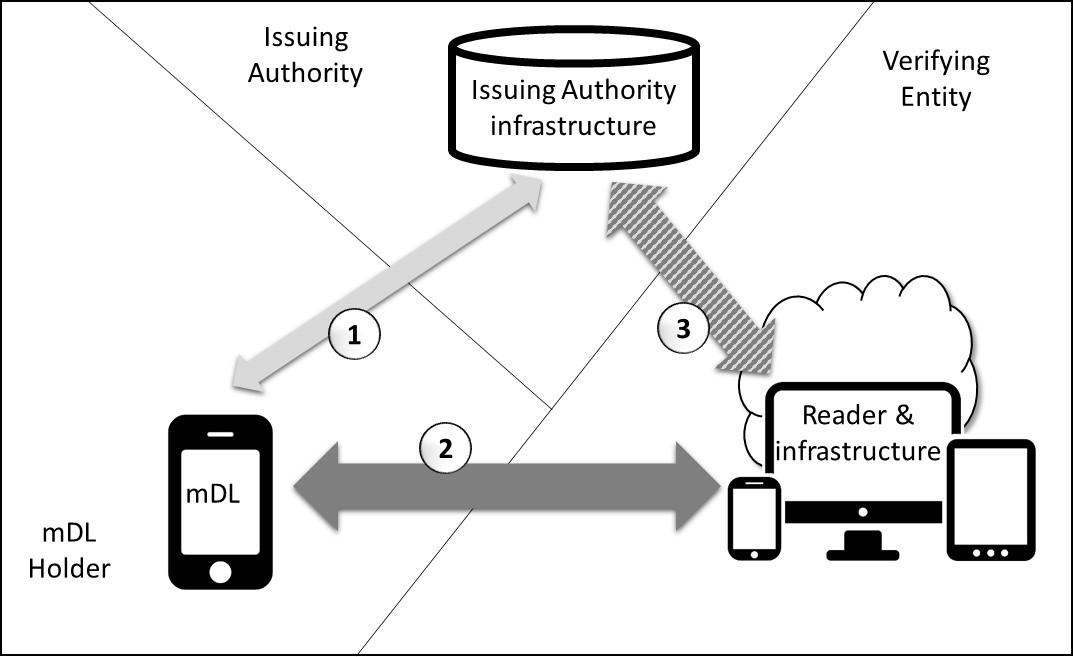
\includegraphics[width=0.8\textwidth]{images/interfaces.png}
	\caption{Ecossistema mDL, incluindo as interfaces associadas}
	\label{fig:interfaces}
\end{figure}
